\def \secname {Solving Ordinary Differential Equations (ODEs)}

\section[\secname]{\hyperlink{toc}{\secname}}


\subsection{Casting Systems  of ODEs in first-order form}

\begin{itemize}
    \item Can always reduce a system of ODEs to a set of first order DEs by introducing appropriate new (auxiliary) variables
    \vspace{10px}
    Example 1:

    \begin{equation}
        y''(x) + q(x) y'(x) = r(x) \qquad '\equiv \frac{d}{dx}
    \end{equation}

    This is second order since the highest derivative is ''

    \item Introduce new variable $z(x) \equiv g'(x) $ then (30) becomes 

    \[ y' = z\]

    \[ z' = r-qz\]

    No derivatives on the RHS

    \vspace{10px}
    Example 2:

    \begin{equation}
        y''''(x) = f(x)
    \end{equation}

    \item Introduce new variables

    \[ y_1 (x) \equiv y'(x)\]
    \[ y_2 (x) \equiv y''(x)\]
    \[ y_3 (x) \equiv y'''(x)\]

    Then (31) Becomes;

    \[ y'=y_1\]
    \[ y_1'=y_2\]
    \[ y_2'=y_3\]
    \[ y_3'= f\]

    \item Thus, generic problem in ODEs is reduced to study of N coupled, \textbf{first order} DEs for functions 

    \[y_i = 1,2,3,... N\]

    \begin{equation}
        y_i'(x) \equiv \frac{dy_i}{dx} (x) = f_i(x,y_1,y_2,...,y_N) \qquad i = 1,2,.., N
    \end{equation}

    Where the $f_i$ are known functions of $x$, $y_i$

    Equivalent forms

    \[\underline{y}'(x) = \underline{f}(x,y)\]

    \[ \underline{\dot{y}}(t) = \underline{f}(t,\underline{y})\]

    dot is the time derivative 
\end{itemize}

Now to actually solve some ODEs we need something else...

\subsection{Boundary/ Initial Conditions}

\begin{itemize}
    \item ODE problem not completely specified by ODEs themselves
    \item Generally, boundary conditions (BCs) are algebraic conditions on the yi in (32) that are to be setastifed at discrete specified points.

    \item Nth order system $\Rightarrow$ need N conditions

    \item BCs divide ODE problems into 2 broad classes:

    
    \begin{enumerate}
        \item Initial value problem
        \item Boundary value problem
    \end{enumerate}
    
    \subsubsection{Initial Value Problems}
    
    \begin{itemize}
        \item  All the $y_i$ are given at some initial value $t_{min}$ (0), wish to find the $y_i$ at some final value $t_{max}$ (or set of values)

        \[ t_n \qquad t_{min} \leq t_n \leq t_{max} \quad n=1,2,...\]

        \item Most relevant for recasting of ODEs in first order form
    \end{itemize}

    \subsubsection{(Two Point) Boundary Value Problems}

    \begin{itemize}
        \item BC's Specified at more than one value of x; 

        typically: some at $x_{min}$, some at $x_{max}$
    \end{itemize}
\end{itemize}

\subsection{Solution of ODEs (Initial Value Problems): Basic Methods}

\subsubsection{Euler Methods}

\begin{itemize}
    \item Consider the basic ODE
    \[ y'(x) = f(x,y)\]

    To be solved on some interval $[x_0, x]$ where $y(x_0)$ is given.
    \item One approach: taylor series

    \[ y(x) = y(x_0) + (x-x_0) y'(x_0) + \frac{(x-x_0)^2}{2} y''(x_0) + \ldots\]

    Where $y'(x_0)=f(x_0,y_0)$
    \item Higher derivatives get messy

    \begin{equation*}
    \begin{aligned}
    y''(x) & = \frac{\partial}{\partial x} f(x,y) + \frac{dy}{dx} \frac{\partial }{\partial y} f(x,y) \\
    & = \frac{\partial f}{\partial x} + f(x,y) \frac{\partial}{\partial y} f(x,y) 
    \end{aligned}
    \end{equation*}
    
    \item Algebraically complicated to go to high order; not \textbf{often} used in practice; good for derivations

    \item Truncate expansion at $O(x-x_0)$
    \[ y(x) \approx y(x_0) + (x-x_0) y'(x_0)\]

    \[ = y(x_0)+(x-x_0)f(x_0,y_0)\]

    where the dx term is equiv to h, i.e. the step size

    \item $\Rightarrow$ Euler Method (forward Euler)

    \begin{equation}
        y(x_0+h) = y(x_0)+h f(x_0, y_0) = y_0 + h f_0
    \end{equation}

    \item Basic algorithm for any ODE integrator: take repeated steps, possibly adjusting step size until integration limit is reached.

    \[ y_{n+1} = y_n + h f_n\]

    \item Accuracy? O(h)

    \item Not recommended for production work

    \item Improve accuracy by using value of y' at mid point of the interval

    \item Want an estimate of $f(x_0+h/2, y(x_0+h/2))$

    \item Compute

    \[ y(x_{mid}) = y_0 + \frac{h}{2} y_0' = y_0 + \frac{h}{2} f_0\]

    \item Modified Euler's method

    \[ y(x_0+h) = y_0+h f(x_{mid}, y_{mid})\]
    \[ x_{mid} = x_0 + \frac{h}{2}\]
    \[ y_{mid} = y_0 + \frac{h}{2} f_0\]

    this is $O(h^2)$ accurate

    \item Improved Euler Method

    \[ y(x_0+h) = y(x_0) + h f_0 + \frac{f(x_0+h, y_0+hf_0)}{2}\]

    Still $O(h^2)$ accurate

    \subsubsection{Improving Euler Methods}

    \begin{itemize}
        \item Taylor Series: use more terms in expansion
        \item Linear Multi-step methods: use data from previous time steps to cancel terms in truncation error
        \item Runge-Kutta methods: use intermediate points within time step

        \item So far we have been looking at:

        \[ y'(x) = f(x,y(x))\]

        \item All methods so far and to come generalize immediately to 

        \[ y_i'(x) = \frac{dy_i}{dx}(x) = f_i(x,y,\ldots, y_N)\]

        for $i=1,2, \ldots, N$

        \[ \mathbf{y}'(\mathbf{x} = \mathbf{f}(x, \mathbf{y}(\mathbf{x}))\]
    \end{itemize}
\end{itemize}

\subsubsection{Runge Kutta Methods}

\begin{itemize}
    \item Modified Euler Methods is an example of a runge-kutta (RK) method of order 2
    \item For any given order, infinite number of distinct RK methods
    \item Very popular example: Fourth order (RK4):

    \[ f_0 = f(x_0, y_0)\]
    \[ f_1 = f(x_0+\frac{h}{2}, y_0+\frac{h}{2}f_0)\]
    \[ f_2 = f(x_0+\frac{h}{2}, y_0+\frac{h}{2}f_1)\]
    \[ f_3 = f(x_0+h, y_0+\frac{h}{2}f_2)\]

    \[y(x_0+h) = y(x_0)+ \frac{h}{6} (f_0 + 2 f_1 + 2 f_2 += f_3)\]

    Here we get $O(h^4)$ accuracy! Good compromise between accuracy and the number of function evaluations.

    \item Non-trivial to derive RK4, but for the case where $f=f(x)$ , can construct it by approximating 

    \[ y(x_0+h) = y(x_0) + \int_{x_0}^{x_0+h} f(x) dx\]

    Integral using Simpson's rule
\end{itemize}

\subsubsection{Adaptive Stepsizes}

\begin{itemize}
    \item In general, want solution of ODEs to some prescribed accuracy

    \item What affects the solution accuracy?

    \begin{itemize}
        \item Step size, h
        \item Accuracy order of method (p)
    \end{itemize}

    \item How do we \textbf{estimate} the solution accuracy?

    \begin{itemize}
        \item Typically estimate \textbf{local} accuracy 
        \item Basic tool: compute solution at $x=x_0+h$ using two different step sizes or methods of different accuracy and then compare them. (HW2 Hint)
    \end{itemize}

    \item How do we control solution accuracy?
    \begin{itemize}
        \item If difference is less than error criterion, accept solution and advance to next time step; otherwise decrease stepsize and repeat integration
        \item If difference is much less than error criterion, increase step size
        \item In practice implement limiters so that stepsizes don't change too much from one time step to another.
    \end{itemize}
\end{itemize}

\subsubsection{Error Control with dual order method}

\begin{itemize}
    \item Two methods (RK, say) with orders of accuracy p, p+1
    \item To leading order, after one step with each method 
    \[ y(x_0+h) = y_{\text{exact}} + k h^{p+1}\]

    p+1 comes from the fact that this is a local error; $O(h^{-1})$ steps to get to any finite time

    \[ \Tilde{y}(x_0+h) = y_{\text{exact}} + \Tilde{k} h^{p+2}\]

    \item Assume h is small; difference between two is

    \[ y(x_0+h) - \Tilde{y}(x_0+h) \approx kh^{p+1} - \Tilde{k}h^{p+2} \approx k h^{p+1}\]

    $\Rightarrow$ direct estimate of the solution error

    \item Typical integrator will use 2 types of error control parameterized by $\epsilon_{\text{ABS}}$, $\epsilon_{\text{REL}}$

    \begin{itemize}
        \item $\epsilon_{\text{ABS}}$: Absolute error control; integrator tries to keep error estimate at/below $\epsilon_{\text{ABS}}$
        \item $\epsilon_{\text{REL}}$: Relative error control; integrator attempts to maintain
        \[\frac{e_{\text{EST}}}{|y(x_0+h)|} \le \epsilon_{\text{REL}}\]
    \end{itemize}

    \item Absolute control: Good when values are O(1) or relatively constant in magnitude or near 0 (numerically ill-conditioned process)

    \item Relative control: good when solution magnitudes vary appreciably 

    \item Can combine two; for example we can say

    \[ e_{\text{EST}} \le \epsilon_{\text{ABS}} + \epsilon_{\text{REL}} |y(x_0+h)|\]

    or \[ e_{\text{EST}} \le \text{MAX}(\epsilon_{\text{ABS}}\text{, } \epsilon_{\text{REL}} |y(x_0+h)|\]

    This is what MATLAB integrators tend to use
\end{itemize}

\subsection{Checking/ Validating results from ODE integrators}

\subsubsection{Monitoring conserved quantities}
\begin{itemize}
    \item Example: for dynamical systems with a Lagrangian/ Hamiltonian, total energy E(t) is conserved

    \item Monitor variation $\delta \hat{E} (t;\epsilon)$ on a solution domain $0 \le t \le t_{max}$

    \[ \delta \hat{E}(t;\epsilon) = \hat{E}(t;\epsilon)-\hat{E}(0;\epsilon)\]

    where $\epsilon \equiv $ error tolerance for integrator 

    \item Should find that $\delta \hat{E}(t;\epsilon)$ is $O(\epsilon)$ 

    \[ \delta\hat{E}(t;\epsilon) = \epsilon g(t) + \ldots\]

    where g(t) is some function

    \item Thus, e.g., if we take $\epsilon\rightarrow\epsilon/10$ should see $\delta \hat{E} \rightarrow\delta\hat{E}/10 $ (approx so long as $\epsilon \gg \epsilon_{\text{machine}}$)
    
\end{itemize}

\subsubsection{Independent residual evaluation}

\begin{itemize}
    \item \textbf{Idea}: Attempt to directly verify that approximate solution (previously y) satisfies the ODEs through the use of an independent discretization of the ODEs (distinct from the one used by the ODE integrator)

    \item Residual $\Rightarrow$ something that should tend to 0 in appropriate limit

    \item Let 

    \[ L[u(t)] \equiv Lu(t) = 0 \]

    where L is a differential operator 

    \begin{itemize}
        \item u(t) can be vector of dependent variables 
        \item most general ODE system 
        \item Assume L linear, but only for convenience
    \end{itemize}

    \item Let $\hat{u}(t;\epsilon)$ be solution computed by ODE integrator at times 

    \[ t^{h} \equiv t_n = t_{min}, t_{min}+h, t_{min}+2h, \ldots, t_{max} \]

    \item Consider second-order centred FDA of $Lu=0$

    \[ L^h u^h = 0\]

    \begin{equation}
        L^h = L + h^2E_2 + O(h^4)
    \end{equation}

    Where E is higher order differential operator (higher than L)

    \item Note that this equation (34) defines $u^h$ and that

    \[ u^h(t) \neq \hat{u}(t^h;\epsilon)\]

    where the u hat term is ODE, integrator

    \item Again, $L^{h}$ can be expanded
    \[ L^h = L + h^2 E_2 + h^4 E_4+ \ldots \]

    Where the E terms are higher order differential operators

    \item Can write

    \[ \hat{u}(t;\epsilon) = u(t) + e(t; \epsilon)\]

    Error in computed solution from ODE integrator

    \item Consider action of $L^h$ on $\hat{u}(t;\epsilon)$

    \[ L^h \hat{u}(\epsilon) = (L+h^2E_2 +h^4E_4+ \ldots ) 
 (u+e(t))\]

    \[ = \cancelto{0}{Lu} + h^2 E_2 u + \ldots L^h e(t)\]
    
    where the last term is small compared to other term


    \[ \Rightarrow L^h \hat{u} \approx h^2 E_2 u = h^2r = O(h^2) \]

    where r is some function

    \[ \text{Assuming \quad } h^2 E_2 \gg L^h e(t)\]

    \item Makeup Monday October 12th 2023

    \item With high accuracy ODE solver is usually possible to satisfy this equation, at least over some time interval $(t_{min}, t_{max})$ and as long as $h$ isn't too small.

    \item KEY idea is to show/check \textbf{correctness} of implementation; e.g. checking for errors in coding of equations
\end{itemize}

\subsubsection{Simple Harmonic Motion Example}

\begin{itemize}
    \item Governing D.E. (unit angular frequency; 0 phase)

    \begin{equation}
        \frac{d^2y(t)}{dt^2} = -y
    \end{equation} 

    \item first order form; define

    \[ y_1(t) \equiv y(t) \qquad y_2(t)\equiv \frac{dy_1}{dt}\]
    \item Then Equation of motion becomes system 

    \[ \frac{dy_1}{dt} = y_2 \qquad \frac{dy_2}{dt} = -y_1\]

    Subject to initial conditions

    \[ y_1(0) = y(0) \qquad y_2(0) = \frac{dy}{dt}(0)\]
\end{itemize}

\textbf{Independant Residual Evaluation}

\begin{itemize}
    \item First rewrite (7) as 

    \begin{equation}
        \frac{d^2y(t)}{dt^2} + y(t) = 0
    \end{equation}

    \item Now, use ODE integrator to generate solution $\hat{u}(t^h;\epsilon)$ on a level-l uniform mesh

    \[ t^h_n = 0,h,2h,\ldots, t_{max}\]

    with 

    \[h=\frac{t_{max}}{2^l}\]

    \item Then apply $O(h^2)$ FDA of equation (36) to $\hat{y}$ to compute residual $R_n$

    \[ R_n \equiv \frac{\hat{y}_{n+1}-2\hat{y}_n+\hat{y}_{n+1}}{h^2} + \hat{y}_n \qquad n=2,3,\ldots , 2^l-1\]

    \item Should find that

    \[ \text{RMS}(R_n) = O(h^2)\]

    \item In particular, compute $R_n$ on 3 separate levels of discretization

    \[ h_1 = h_e\]
    \[ h_2 = 2h_1 = h_{l-1}\]
    \[ h_3 = 4h_1 = h_{l-2}\]

    But using single level-l calculation using the ODE integrator

    \item Then by Plotting 

    \[ 16R^l, \quad 4R^{l-1}, \quad R^{l-1}\]

    On a single graph, should see near-coincidence of the curves $\Rightarrow$ convergence of independent residual.
    
\end{itemize}

\subsection{Passing Additional Arguments to the Derivatives Function}

\begin{itemize}
    \item Systems of ODE often have additional parameters (Change from solution to solution)
    \item The calling sequence for the derivatives function is fixed

    \[ \text{function derivative } = \text{odefun}(t,y)\]

    \item Need mechanism to pass in additional information
    \item At least 3 ways

    \subsubsection{Use an anonymous function definition}

    \begin{itemize}
        \item Example: 3 Parameter a,b,c
        \begin{verbatim}
        code function    odefun(t,y,a,b,c)
        a=1.0
        b = 2.5
        c =3.14
        [tout yout] = ode45(@(t,y) odefun(t,y,a,b,c, ... tspan, yphi)
        \end{verbatim}
    \end{itemize}

    \subsubsection{Use a Global Variable}
    \begin{itemize}
        \item Be default, scope of matlab variable is local to programming unit (Script, function)
        \item Change this behaviour by using global command
        \item Must use declaration in all programming units in which we want access to variable

        \begin{verbatim}
            % Script; function-caller
                .
                .
                .
            global m;
            m = 1.56;
                .   
                .
                .
            [you yout] = ode45(@fcn, [0.0 1.0], [0.0 2.0]);
                .
                .
                .
            function derivs = fcn(t,y)
                global m;
                    .
                    .
                    .
            end
        \end{verbatim}

        \item Syntax for multiple global variables:

        \begin{verbatim}
            global a b c;
        \end{verbatim}

        Note: no commas
    \end{itemize}

    \subsubsection{Adjoin parameter to ODE system}

    \begin{itemize}
        \item Treat any parameter as a \textbf{dependent} variable with a trivial governing ode
        \item for example 
        \[ \frac{dm}{dt} = 0 \qquad m(0) = 1.56 \Rightarrow m=\text{const} = 1.56\]

        \item A bit more computationally intensive than the other two approaches; and a bit more complicated to implement.


        $\Rightarrow$ (Matt) Advocates using anonymous functions (although he uses global variables).
    \end{itemize}

    \item See example of dumbbell orbit slides from the course site
\end{itemize}

\subsection{The one dimensional Toda Lattice}

(following https://www.mat.univie.ac.at/~gerald/ftp/book-jac/toda.html)\newline

Model for crystal (simple solution), particle sites with spring between sites:

\[ . \quad . \quad . \quad . \quad . \quad . \quad . \quad . \quad . \quad . \quad . \quad . \quad .\]

with nearest neighbour interactions

\begin{itemize}
    \item Let g(n,t) be displacement of particle n from its equilibrium position; p(n,t) its momentum (m=1) and V(r) the interaction potential where r is the interparticles separation.

    \item Hamiltonian

    \[ \mathcal{H} (p,q) = \sum_n \frac{p(n,t)^2}{2} + V(q(n+1,t)-q(n,t))\]

    \item Example: Harmonic Interaction

    \[ V(r) = r^2\]

    \item Resulting set of equations are linear, with constant set of coefficients

    \item Solution: super position of normal modes

    \item \textbf{Solitons}: pulse like waves which propagate and interact similarly to particles
    \item \textbf{Nonlinear}: Dispersion balances non linearity (Focusing)
    \item Motivation in part by soliton theory, TODA (1967) came up with a potential 

    \[ V(r) = e^{-r} + r-1\]

    where the r-1 term means we get harmonic behaviour in small r limit

    \item Equations of Motion:

    \[ \frac{d}{dt} p(n,t) = e^{-(q(n,t)-q(n-1,t))}-e^{-(q(n+1,t)-q(n-1,t))}\]

    \[ \frac{d}{dt} q(n,t) = p(n,t) \qquad n=1,2,\ldots, n_{sites}\]

    \item Can show that the following is a solution

    \[ q_1(n,t) = q_+ + \log (\frac{N}{D}\]

    \[ N = 1+ \frac{\gamma}{1-e^{-2\kappa}} \text{exp}(-2\kappa n + 2 \sigma \sinh (k) t)\]

    \[ D = N \qquad \text{BUT} \qquad n\rightarrow n+1\]

    \item Can put some example values in like
    \[ \kappa = \gamma  = q_+ = 1.0 \qquad \text{and} \quad \sigma = 1\]
    and we get a "kink" solution (looks like heaviside function sorta)

    \item Propogrates to the right is sigma is +1 and left if sigma is -1

    \item Speed of propagation is $\sinh(\kappa)/\kappa \Rightarrow$

    Thinner kinks travel with higher speeds

    \item Refer to Slide on Course Site for ODE MATLAB Implementation of this Toda Lattice Problem
\end{itemize}


\textbf{October 18th 11:07am}

\textbf{THE VAN DER POL OSCILLATOR }\newline 


(following Tsatsos ...)

\begin{itemize}
    \item 1920s Van der Pol (VdP) experimented with oscillations in a vacuum tube triode circuit
    \item Concluded that all initial conditions converged to some finite-amplitude periodic category
    \item Proposed a non-linear ODE to model phenomena
    \item (unforced VdP equation)
    \begin{equation}
        \frac{d^2x}{dt^2}+ a(x^2-1) \frac{dx}{dt} + x = 0
    \end{equation}
    Where a is constant (parameter) and when a=0 we get linear oscillator

    \item Version of equation 37 here that includes forcing term

    \[ \frac{d^2x}{dt^2} + a(x^2-1) \frac{dx}{dt} + x = b s\sin(\omega t)\]

    where $b$ and $\omega$ are parameters (constants)

    \item Model has application in: physics, electronics, biology, neurology, sociology, economics
    \item view VdP equation as "typical" nonlinear dynamical system; illustrates some of qualitative ways we can describe such systems
\end{itemize}

\subsubsection{Analysis Methods}
\begin{enumerate}
    \item \textbf{Phase Space Plots}: Good for 2-D systems (one x, one p (dx/dt); plotting trajectories in phase space $\Rightarrow$ reveal nature of dynamics

    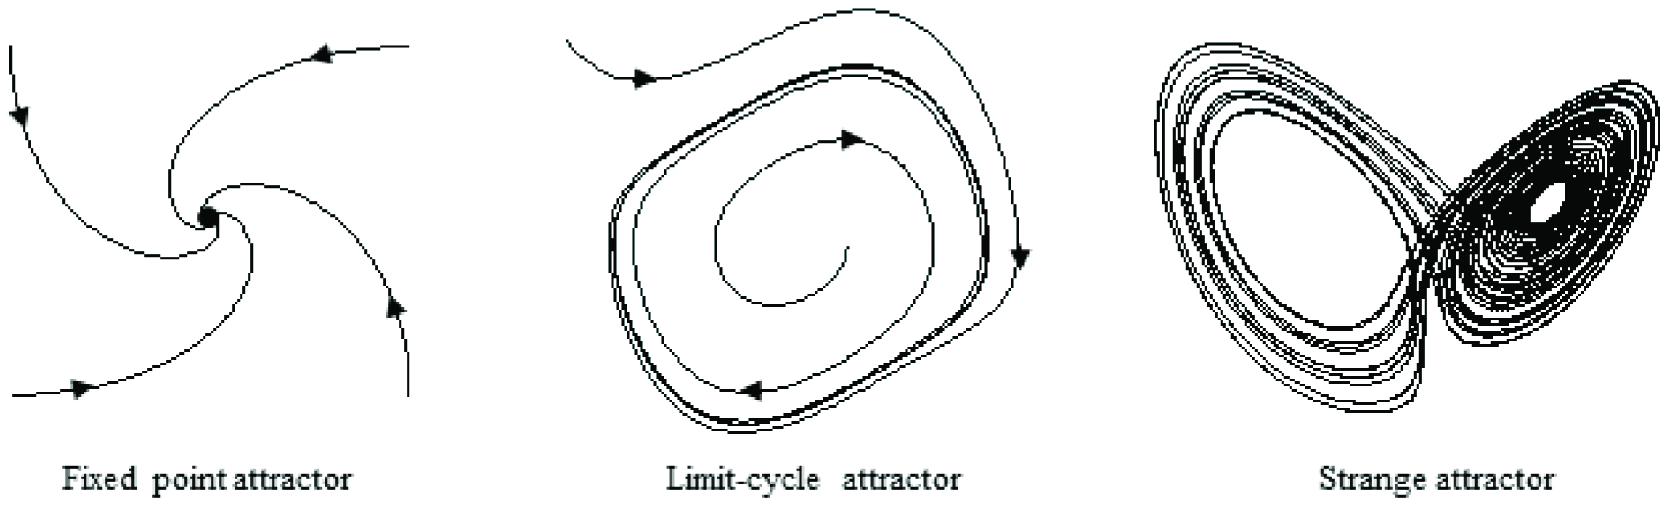
\includegraphics[width = \linewidth]{Images/attractor_types.png}
    

    \item Nature of long-time attractors

    \begin{enumerate}
        \item \textbf{Fixed Point:} trajectory converges to a single point in phase space
        
        \item \textbf{Limit Cycle}: (Periodic Trajectories) Trajectory converges to closed curve in phase space (undamped oscillator)
        
        \item \textbf{Strange Attractor}: Trajectory converges to "curve" with fractional dimension in phase space \newline 

        Coastline structure on all scales 

        \[ l \approx x^{(d-1)} \qquad 1 \le d \le 2 \]
        
    \end{enumerate}

    \item \textbf{Poincare Section:} view dynamics periodically sometimes projecting onto a space with reduced dimensionality (1d on 2d typically) for case of driven dynamics, natural period is period of forcing. Resulting trace of dynamics is called Poincare section. Various features can appear

    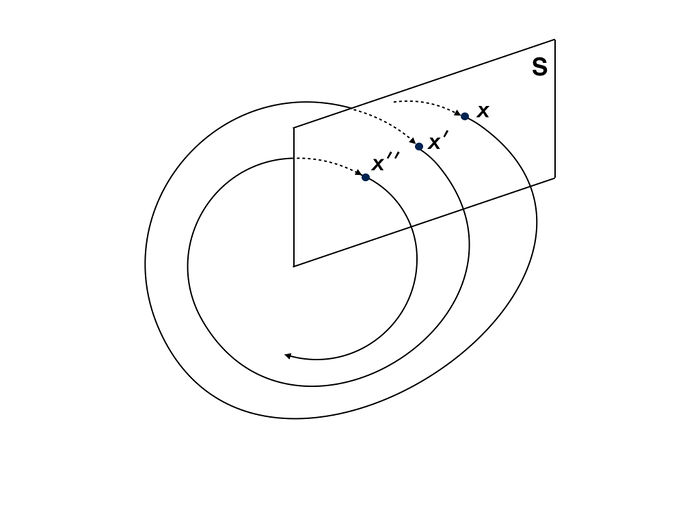
\includegraphics[width = \linewidth]{Images/poincare_section.jpg}

    \begin{enumerate}
        \item Fixed Points: single points on Poincare section
        \item Limit Cycles: will appear as one or more isolated points
        \item Almost periodic trajectory: will appear as a near-continuous curve
        \item Chaotic dynamics: will appear as a "curve" with fractional dimensions
    \end{enumerate}
    \item Bifurcation Diagram \newline
    
    Plots which show dependence of Poincare section on a problem parameter typically, plot a certain number of points in a given Poincare section, as a function of the parameter \newline 

    Typical use here; show transition to chaos (period doubling for example)

    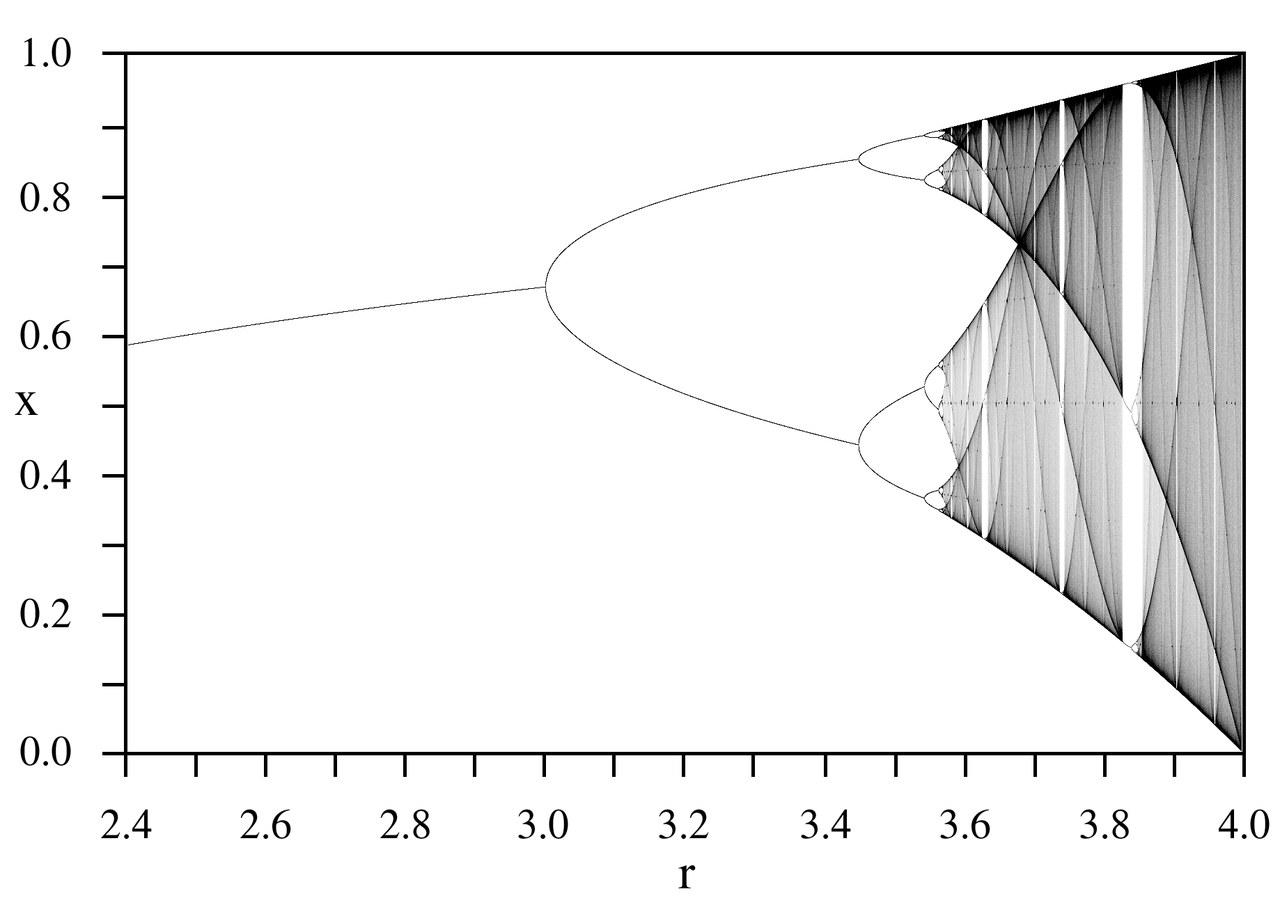
\includegraphics[width = \linewidth]{Images/bifurcation_diagram.png}
\end{enumerate}

\textbf{October 20th 2023, 11:00am}

\subsection{Boundary Value Problems - Shooting}

\begin{enumerate}
    \item Introduction \newline
\end{enumerate}

Recall: 2-PT Boundary value problems; B.C.'s supplied at two points - typically end points of the solution domain
\begin{itemize}
    \item In idealized physical problems, one of the points will often be $x = \infty$

    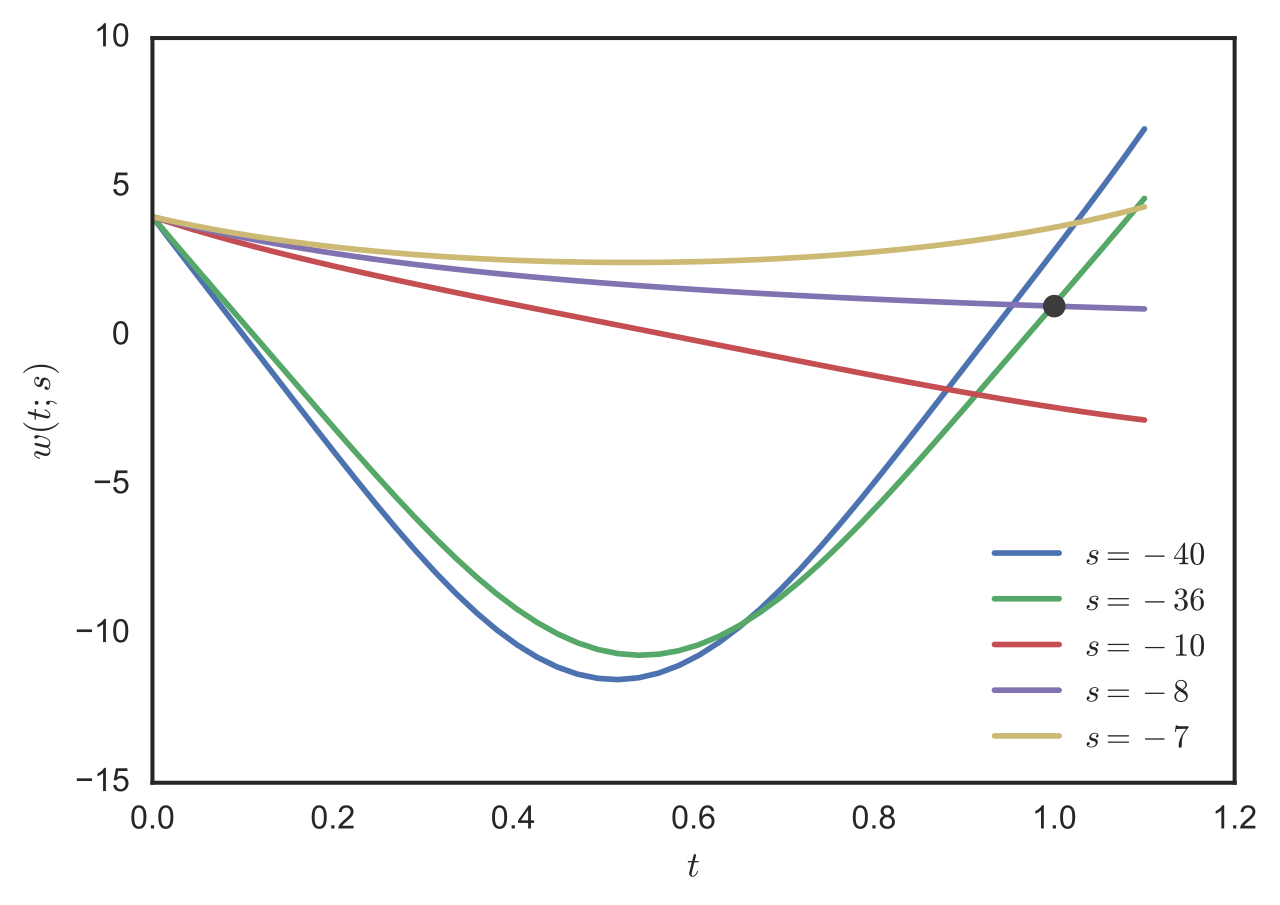
\includegraphics[width = 0.8\linewidth]{Images/shooting_ode_bvp.png}
    \item * Refer to SOLVING BVPs WITH THE ode45 INTEGRATOR AND SHOOTING* slides

\end{itemize}

End of the ODE section! \newline

\textbf{Monday}
